\documentclass[a4paper, 12pt]{report}
\usepackage{graphicx}
\usepackage[backend=biber,style=alphabetic,sorting=ynt]{biblatex}
\usepackage{blindtext}
\usepackage{hyperref}
\usepackage{xurl}
\usepackage{amsmath}
\usepackage{bm}
\usepackage{float}
\usepackage{tabulary}
\usepackage{array,etoolbox}
\graphicspath{ {./images/} }
\addbibresource{citations.bib}

\begin{document}
\begin{titlepage}
    \begin{center}
        \vspace*{1cm}

        \Large{
            \textbf{matsubara}
        
            \textbf{Case-based Recommendation for \\ Music Playlists}
        
            \vspace{0.5cm}
        
            \textit{Alexander Stradnic}
        
            \vspace{3cm}
        
            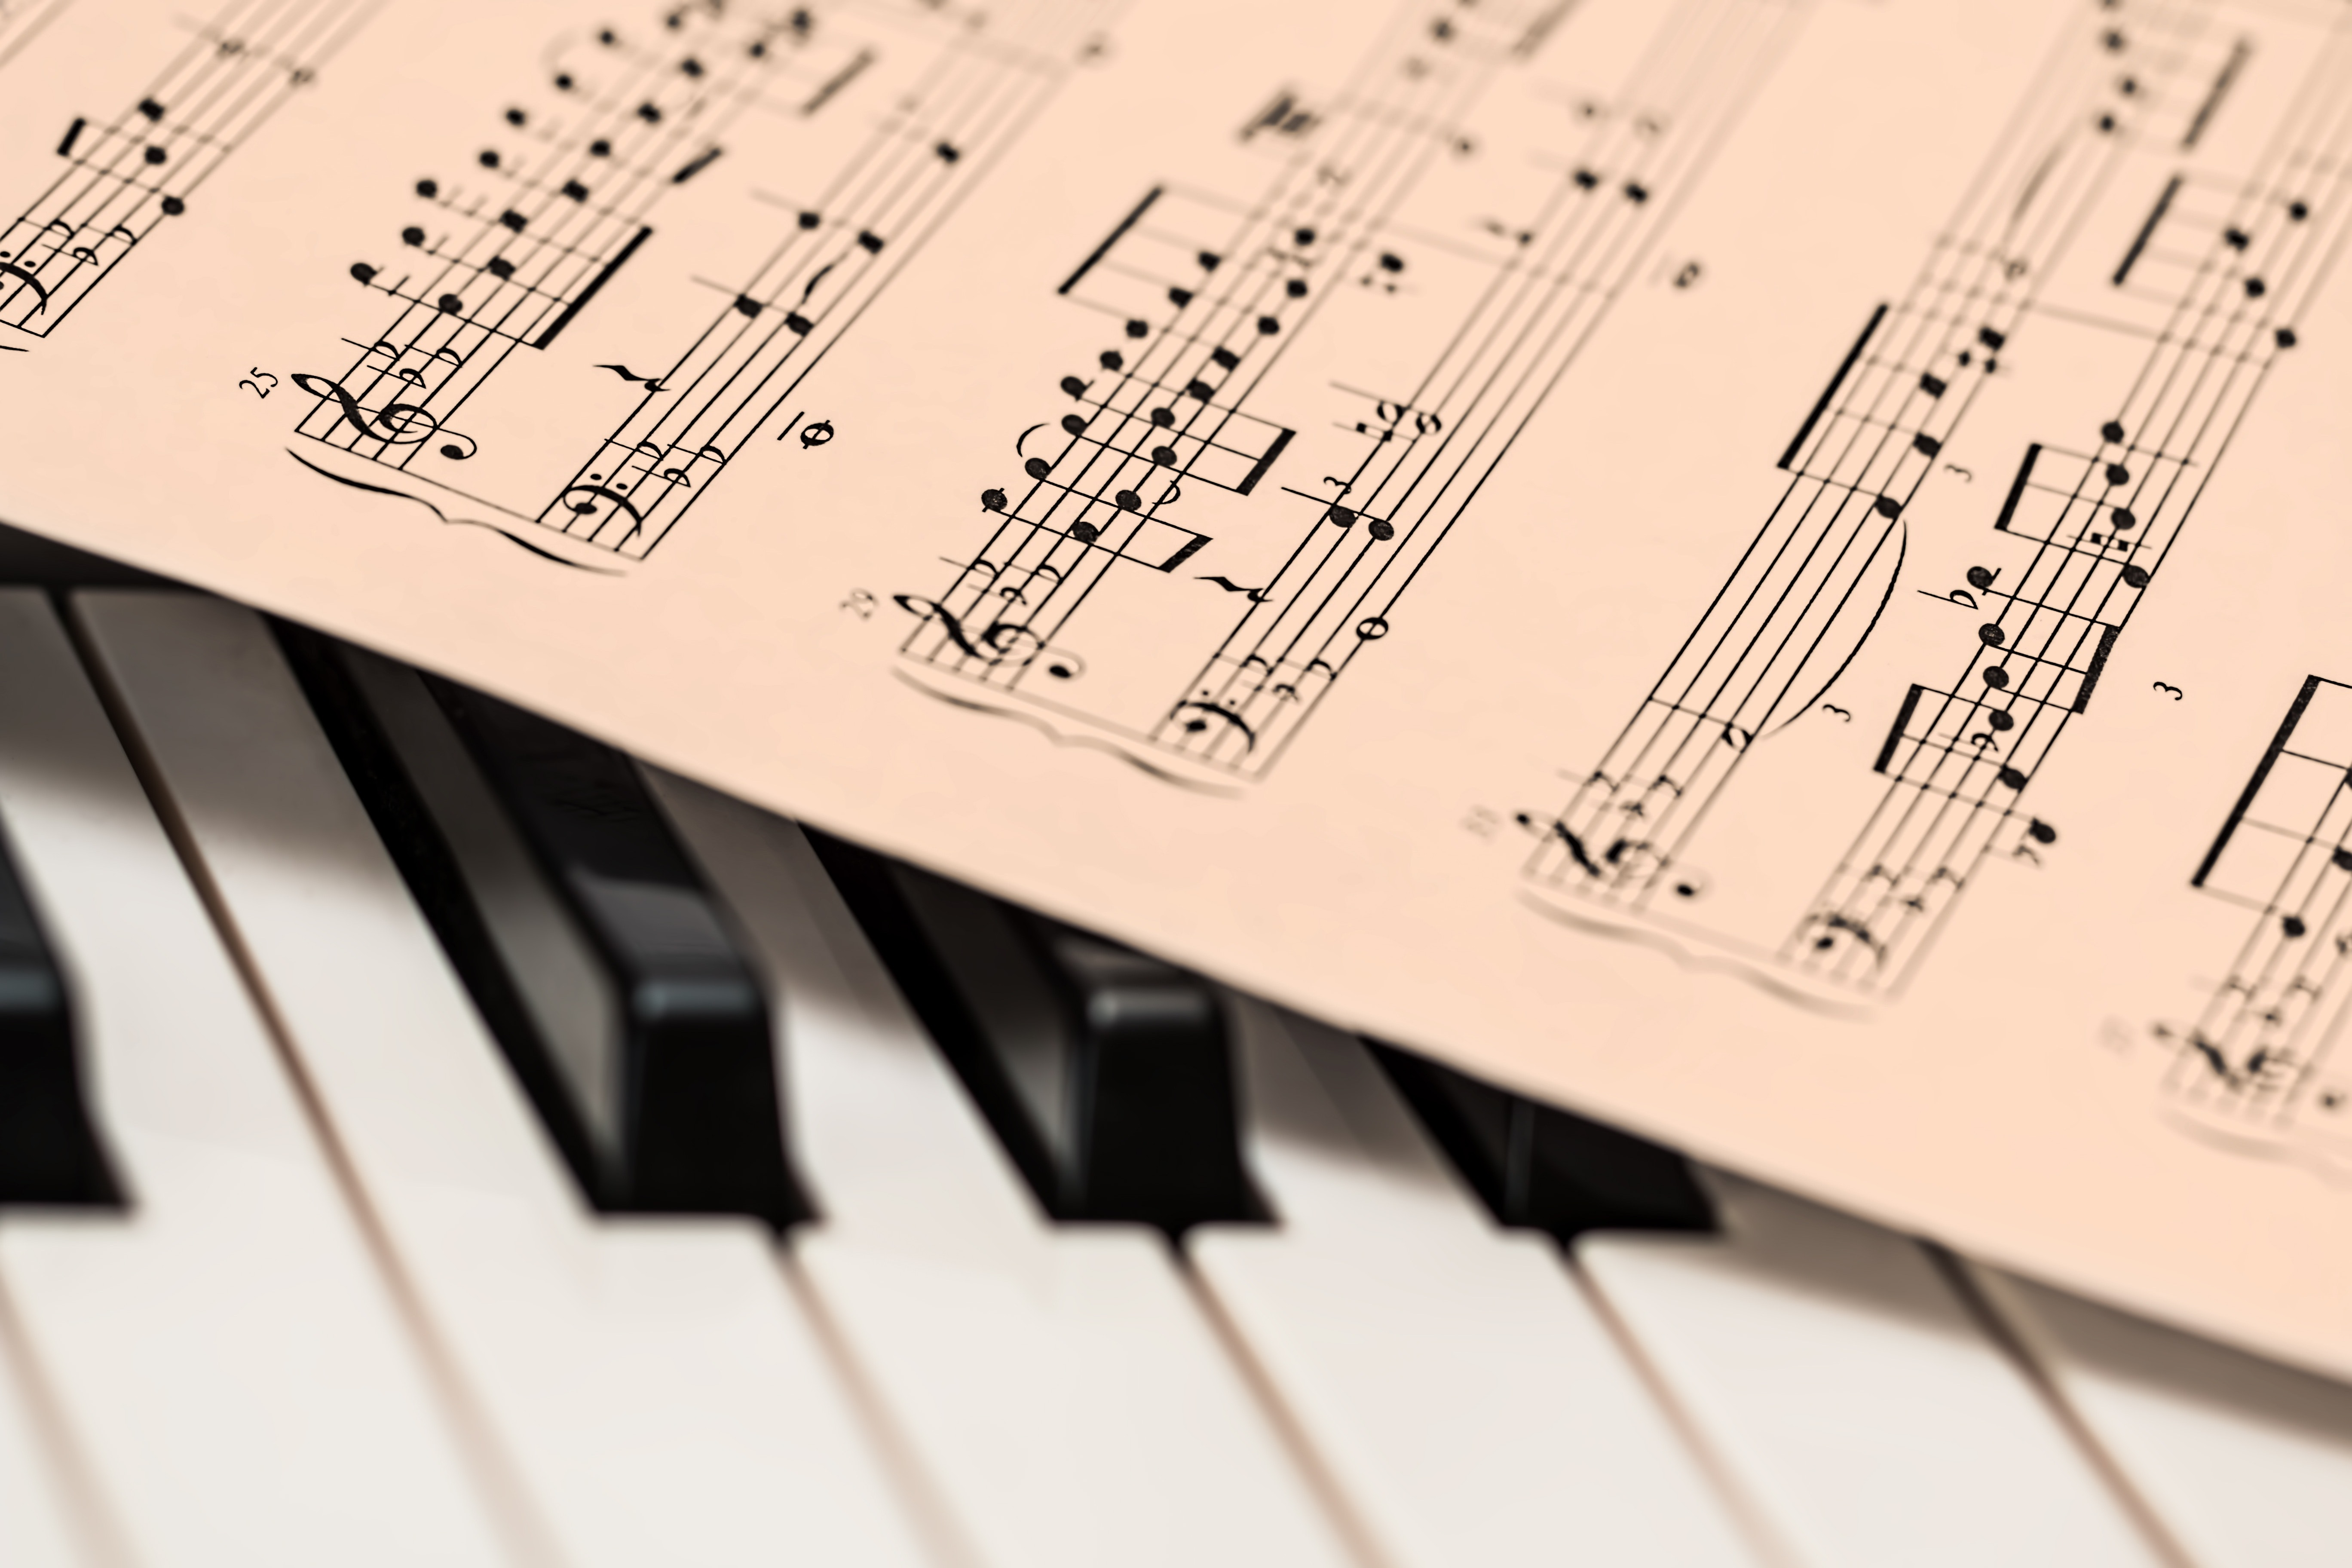
\includegraphics[width=0.6\textwidth]{piano.jpg}
        
            \vspace{3cm}
        
            \textit{Prof. Derek G. Bridge}
        
            \vspace{0.5cm}
        
            \textbf{University College Cork}
        
            \textbf{Final Year Project, BSc. Computer Science}
            
            \textbf{April 2023}
        }
    \end{center}
\end{titlepage}

\chapter*{Abstract}
In this Final Year Project I present the use of Case-based Recommendation in creating music playlists, 
along with providing an implementation of this CBR system and examples of output.
Playlists are sequences of songs arranged in a particular order. Using this information, 
context can be gained from previous playlists in order to build a new playlist from a given seed song. 
Patterns in previous playlists can be analysed and used to create an enjoyable and coherent listening experience.

\chapter*{Declaration of Originality}
In signing this declaration, you are conforming, in writing, that the sub-
mitted work is entirely your own original work, except where clearly at-
tributed otherwise, and that it has not been submitted partly or wholly for
any other educational award.
I hereby declare that:
\begin{itemize}
    \item this is all my own work, unless clearly indicated otherwise, with full and proper accreditation;
    \item with respect to my own work: none of it has been submitted at any educational institution contributing in any way to an educational award;
    \item with respect to another's work: all text, diagrams, code, or ideas, whether verbatim, paraphrased or otherwise modified or adapted, have been duly attributed to the source in a scholarly manner, whether from books, papers, lecture notes or any other student's work, whether published or unpublished, electronically or in print.
\end{itemize}
\large{\textbf{Signed:}} \raisebox{-.2\height}{
\includegraphics[width=150pt]{signature.png}} \\
\large{\textbf{Date:}} 12th April 2023

\tableofcontents


\chapter{Introduction}

\section{Music Listening in the Pre-Industrial Era}
Throughout most of history, the only way for a person to listen to a piece of music was to either attend a live performance,
or perform themselves. While the written recording of music as notation has existed for hundreds of years, the majority of the population 
would not have the education and time to be able to read and reproduce this music, aside from the nobility who would have 
court musicians writing and performing music for them. W.A. Mozart, one of the most well-known composers today, had to travel the courts of Europe 
after leaving Salzburg due to low pay and the desire to compose more freely; he battled with financial insecurity throughout his life.
Turlough O'Carolan was a famous blind harper who traveled across Ireland composing planxties for patrons.

This also generated a rift between the 
organised, written music of the elites with professional performers,
compared to more accessible folk/traditional music of the populace which could be performed solo or by a group, and was passed down by ear.

\section{Early Sound Reproduction}
Attempts to reproduce the sound of music have been attempted and improved as technology has advanced,
beginning with spring-wound machines in which a metal pin strikes a series of raised pitches on a rotating cylinder or disc.
Music boxes are the most well-known, and reproduce a single melody line, though more complex contraptions automatically playing flutes,
violins and keyboard instruments also existed, and player-pianos continue to exist, though less common and usually digitally operated.

The issue with these machines is that they would play exactly as inscribed, and with simplistic musicality. They tended to be large, expensive and limited to few tracks.

\section{19-20\textsuperscript{th} Century Innovations}
With the development of early cylinder-based phonographs, followed by disc-based gramophones, allowed the widespread recording of music to occur.
Gramophone recording would inscribe the sound vibrations onto a master record, from which copies would be printed onto shellac-based, and later polyvinyl-based
discs. These discs were analog recordings of actual artist performances and improved in clarity with advances in materials and recording techniques.
Acoustic recording gave way to electronic with microphones allowing more control and flexibility.
Later on, magnetic tape recording was invented, and while initially only used in studio recording,
eventually allowed for a small, portable and rugged music format to be developed in the form of the cassette,
which started being produced from the 1960s and became more popular into the '70s.

Towards the end of the 20\textsuperscript{th} Century, digital solutions to storing and playing music were explored, with the Compact Disc exploding onto the scene in 1982,
effectively replacing any market share records had remaining, and competing with compact cassettes, replacing them for audio playback in the 2000s.

\section[Music Ownership, Albums and The Computer Age]{Music Ownership, Albums and \\ The Computer Age}
Until the rise of computers and the Internet, the way in which people listened to recorded music was starkly different. One would listen typically hear a song on the radio or live, and,
if they wished to listen to it repeatedly, would visit the record store and purchase a copy of the song on vinyl, cassette, or CD. 
Cassettes also allowed for radio streams to be recorded.

They could also purchase a collection, typically an album on the medium of their choice, which would tend to be better value.
In many styles of music such as pop and rock, collections of pieces or songs would be released together by an artist in albums.
Music albums, initially inspired by photo albums, typically comprise a collection of tracks which tend to cover a theme or idea, and are intended by the artist to be listened sequentially.
Even in other genres, music would be grouped and sold, length depending on the format and album. This allowed for longer uninterrupted listening before the
listener would have to change the disc or cassette manually or with a suitable player.

The practice of ``owning'' your own music would continue to remain popular with many people until the advancement of Internet infrastructure and services.
Apple pioneered the digital sale of music online, allowing songs to be purchased individually, to be played on MP3 players such as the iPod.
This broke with the previous paradigm of selling and playing by the album. People now had the ability to create their own custom collections of songs called playlists.
At this point, most people still consciously which songs to purchase, and gathered their own personal collections on their own.
However, with the rise of Napster and later Spotify, this model of music ownership becamse less popular, as people wished to listen to more music without having
to purchase every single song they wanted to listen to. Apple iTunes also started facilitating streaming, leading us to today, where most stream music 
from a platform such as YouTube, iTunes, or Spotify.

\section[Modern Problems Require Modern Solutions]{Modern Problems Require Modern \\ Solutions}
This rise in music streaming, along with the ability to purchase individual songs for a cheap price, has meant that listening to albums from start to finish
drastically reduced in popularity. Many people listen to playlists or just the individual songs themselves as shown in these surveys
carried out by Deezer\textsuperscript{\cite{deezer}} and MusicBiz\textsuperscript{\cite{musicbiz}}.

A major convenience offered by music streaming providers nowadays is the automatic generation of playlists,
making it easier for users to listen to a variety of music without having to create their own playlists manually.
This is now done using many methods ranging from popularity counts (seen in many services as the ``Hot'' or ``Trending'' pages) to personalised user-user and user-item algorithms,
which take into account previous user listening activity and the preferences of ``similar'' users. Thus the problem: \textit{Which
methods generate the most interesting playlists for users?} In this paper, I explore various ways of generating music playlists, focusing on case-based recommendation.




\chapter{General Implementation Details}

\section{Data}
The data was acquired from Spotify's Million Playlist Dataset. Other options explored were MusicBrainz and the Million Song Datasets,
which have various metadata tags available for songs and artists, but were dropped due to lack of source playlists.

Processing was done on the dataset running in SQLite.
The data was downloaded from Spotify's servers, structured as a set of JSON files.
This was then converted into an SQLite database to improve lookup performance.
Additional data was queried from Spotify's API.

\section{Tables}
\begin{itemize}
    \item \texttt{tracks} -- specific track info, song name, album name, etc.
    \item \texttt{track\_features} -- generic track features as measured by Spotify such as acousticness, danceability, speechiness etc.
    \item \texttt{artist\_genres} -- artists and their associated genres
    \item \texttt{playlists} -- playlist information
    \item \texttt{playlist\_tracks} -- link between tracks and playlists
    \item \texttt{seq2\_simple} -- all sequences of \(\langle song1, song2 \rangle\), usually aggregated in processing
    \item \texttt{similarities} -- artist similarity rating based on their genres
\end{itemize}

\section{Processing}
The implementations are written in \emph{Python}.
This is due to the large amount of useful libraries available for the language such as \emph{Numpy}, as well as the quick 
writing and readability. 

\section{Output}
All algorithms described in this paper take in an input seed track URI, and output a generated list of track URIs.
\\
\\
\texttt{(spotify:track:1, spotify:track:2,\ldots, spotify:track:\(\lambda\))}

\section{Limitations: Song Output}\label{section:limsongs}
Due to the nature of Case-based Recommendation, it can only generate playlists containing songs that are already present in the seed dataset, 
thus limited to songs up to 2017.
This is because it ranks songs rather than a generic set of features, and even an output comprising a list of feature sets would be limited to the dataset
due to the inability of querying Spotify by features.

The similarity-based approach likewise only works for precomputed similarities in the dataset.

\section{Limitations: Personalisation}\label{section:limpersonalisation}
Personalising songs and genres based on a Spotify User Profile is technically possible by preferring user playlists and song features
over generic playlists, it was beyond the scope of this project, requiring user authentication, processing and further development of the demonstration \hyperref[chap:webapp]{web-app}.
User-user recommendation and weighting is also theoretically possible, but would require manual input of other users as Spotify does not have a
public API for getting ``similar users''.



\chapter{Similarity-based Solutions}
\section{Background}
A logical conclusion one would come to when asked how to generate a playlist given an input song would be to create a playlist of similar songs.
In fact, there are many websites that generate playlists based off a song such as \href{https://www.chosic.com/playlist-generator/}{Chosic}, \href{https://spotalike.com/}{Spotalike}
and \href{https://www.similarsongfinder.com/}{SimilarSongFinder}. These tend to be used by users to discover new artists and songs.

\section{Simple Similarity}
One method to create playlists is to simply choose the most similar song to the given song.
The next most similar song to that song, aside from any songs already in the playlist, is then added.
This process can be continued until the playlist of desired length is generated.

\section{GLSF}
An interesting solution utilising similarity is the Global-Local Similarity Function\textsuperscript{\cite{glsf}}. In this approach, a playlist is generated
in which the transition between tracks is constrained by the difference in track features between the songs in order to prevent a hard transition between two songs.
The transitions are measured by scoring functions and songs with scores in the desired range are chosen.

\section{Conclusion}
Similarity rating is a simple but powerful concept. It has many applications and can be used as a building block in more advanced algorithms
or be the core of an algorithm as with GLSF. In this project I chose to implement a simplistic version of similarity, mainly as a reference against
the various Case-based configurations\textsuperscript{\ref{chap:casesolutions}}.



\chapter{Similarity-based Development}\label{chap:simdev}
\section{Design}
Based on the data available, I decided to design the algorithm to output a playlist with songs chosen randomly from an artist not already in the list.
While I wanted to work based on the songs themselves, the artists actually contained the features, so the algorithm works using artist similarity.
The seed song's artist is looked up and the most similar artist is chosen. A random song by that artist is chosen.
The most similar artist to the previously chosen artist not already in the list is then chosen and the process is repeated until a playlist of desired length is achieved.

\paragraph{Jaccard Similarity}
\[Sim(\bm{s_1}, \bm{s_2}) = \frac{|\bm{s_1} \cap \bm{s_2}|}{|\bm{s_1} \cup \bm{s_2}|}\]

\section{Implementation}
The implementation queries a table which contains the similarity score between all artists' genres and chooses the highest ranked artist to the initial song's artist.
It then continues as described above, outputting a list of tracks.

Another implementation utilising similarity between artist tags along with genres was written for the Million Song Dataset, but does not output Spotify URIs.



\chapter{Similarity-based Testing}
All similarity-based playlists generated started with the original seed song, generating as described in Development\textsuperscript{\ref{chap:simdev}}.
A drawback to my approach is that since it is based off of artists, it can only have one random song per artist in the list.

\section{Examples}
\paragraph{A standard playlist of length 10.}
\preto\tabular{\setcounter{magicrownumbers}{0}}
\newcounter{magicrownumbers}
\newcommand\rownumber{\stepcounter{magicrownumbers}\arabic{magicrownumbers}}
\begin{center}
    \begin{figure}[H]
        \begin{tabulary}{\linewidth}{|@{\makebox[2em][c]{\rownumber}}|L|L|} 
            \hline
            \textbf{TOTO} & \textbf{Hold the Line} \\
            \hline
            Dary Hall \& John Oates & You've Lost That Lovin' Feeling \\ 
            \hline
            Fleetwood Mac & Got to Move \\
            \hline
            Meta Loaf & Good Girls Go To Heaven \\
            \hline
            Dire Straits & Telegraph Road \\
            \hline
            Foreigner & Growing up the Hardway \\
            \hline
            Journey & Lights \\
            \hline
            Boston & You Gave up on Love (2.0) \\
            \hline
            Styx & Light Up \\
            \hline
            Kansas & The Pinnacle \\
            \hline
        \end{tabulary}
        \caption{\url{https://open.spotify.com/playlist/4qShHvmJIaFat9wV2yTgUK}}
    \end{figure}
\end{center}

\paragraph{A playlist of length 20, 11--19 are skipped for brevity.}
\begin{center}
        \begin{figure}[H]
        \begin{tabulary}{\linewidth}{|C|L|L|} 
            \hline
            \rownumber & \textbf{George Michael} & \textbf{Careless Whisper} \\
            \hline
            \rownumber & Cher & Fires of Eden \\ 
            \hline
            \rownumber & Mandy Moore & Want You Back \\
            \hline
            \rownumber & Hannah Montana & Don't Wanna Be Torn \\
            \hline
            \rownumber & Zac Efron & Ladies' Choice (``Hairspray'') \\
            \hline
            \rownumber & Kesha & Blow -- Deconstructed Mix \\
            \hline
            \rownumber & Demi Lovato & Confident Outro/For You Intro \\
            \hline
            \rownumber & Christina Aguilera & When You Put Your Hands on Me \\
            \hline
            \rownumber & Liam Payne, Quavo, Nevada & Strip That Down -- Nevada Remix \\
            \hline
            \rownumber & Hailee Steinfeld, Grey, Zedd, KillaGraham & Starving -- Killagraham Remix \\
            \hline
            \ldots & \ldots & \ldots \\
            \hline
            20 & Ashley Tisdale & Acting Out \\
            \hline
        \end{tabulary}
        \caption{\url{https://open.spotify.com/playlist/1ocr27MzrILNfgpHznMVKn}}
    \end{figure}
\end{center}

\section{Compute Time}
Playlists of length 10 were created, with the time to return a result for each captured below. The time to create a playlist based on similarity took on average 18 seconds.

\begin{center}
    \begin{figure}[H]
        \begin{tabulary}{\linewidth}{|C|C|C|} 
            \hline
            TOTO & Hold the Line & 18.002 \\
            \hline
            George Michael & Careless Whisper & 17.947 \\
            \hline
            Jonathan Parecki & Miiro (From ``KanColle: Kantai Collection'') &  18.006 \\
            \hline
            Britney Spears & Toxic & 17.971 \\
            \hline
            PSY & Gangnam Style & 17.959 \\
            \hline
        \end{tabulary}
    \caption{List of seed songs and times to compute playlists}
    \end{figure}
\end{center}

\section{Conclusion}
Similarity allows for a quick way to generate playlists from a seed song but may be inconsistent in the quality due to the random choice of song from each artist.
Artists tend to produce more than one type of music, but unfortunately many songs were missing genre descriptors.

\chapter{Case-based Solutions}\label{chap:casesolutions}
\section{Background}
Case-based solutions extrapolate sequences and patterns from input user data.
The outcome of this analysis is then used when it is queried to generate a new output.
There are many applications of case-based recommendation, from advising select products based on price and features to recommending restaurants and services\textsuperscript{\cite{cbr-general}}.

\section{Application to Playlist Generation}
As demonstrated in the paper by Baccigalupo and Plaza\textsuperscript{\cite{main}}, it is possible to adapt case-based reasoning to generate playlists in various forms.
In this project I design a case-based algorithm using user-generated playlists from Spotify, and expand on work done prior by testing various settings of parameters.



\chapter{Case-based Design}\label{casedesign}
\paragraph{Case-based Recommendation (CBR):}
The approach in which a playlist is generated from a seed song/shorter playlist using sequential patterns 
learned from a dataset of existing playlists.
CBR is a method of recommendation which can be used in contexts in which a meaningful order or sequence to objects is desired or useful.
There can also be a large variety of possible values (such as songs in this case).

\section{Case Base}
A set of playlists may then be filtered to remove meaningless and/or noisy playlists, forming the Case Base.
The playlists are then analysed, using their song order as well as the songs themselves, in order to 
come up with new playlists to generate from an initial seed song.

\section{Retrieval of Playlists}
From this Case Base of playlists \(\mathcal{C}\), two main values are computed for each playlist:
\begin{itemize}
    \item The Attribute Variety: How varied and diverse the playlist is, based on song attributes
    \item The Coherence of the playlist: How relevant the sequences are to the seed song, as well as how many
\end{itemize}

After computing the Variety and Coherence for each playlist \(p\in\mathcal{C}\), a rating function combines both and allows the playlists to be ordered.
\[\rho(p, s) = Var(p) \cdot Coh(p, s), \forall p \in \mathcal{C}\]

\section{Reuse}
After the \(k\) playlists have been ranked, they have to be then converted in some way to form a single playlist of a particular length \(\lambda\). 
This is to be done using a process called Constructive Adaptation\textsuperscript{\cite{constructive-adaptation}}, which comprises of two parts:
\begin{enumerate}
    \item Hypothesis Generation(HG): How partial solutions are extended from the currently generated state of the playlist 
    (either the seed song at the beginning or the highest ranked generated sequence chosen by HO afterwards)
    \item Hypothesis Ordering(HO): Uses the ranking of sequences from \(\mathcal{C}\) to rank the list of newly generated playlists after each iteration of HG
\end{enumerate}
An ideal solution is generated by appending or prepending a song at a time to the seed song, decided but creating potential successor 
solutions using Hypothesis Generation and ranking using Hypothesis Ordering. 
This is continued recursively down the most ideal node. However, if no successor solution is generated at a particular level, then it is discarded from the 
list of ranked generated sequences, and the process continues from that point, until a playlist of length \(\lambda\) is generated.

\section{Formulae Used\textsuperscript{\cite[pp. 5--10]{main}}}
\paragraph{Variety}
The variety of each playlist in \(\mathcal{C}\) is calculated based on the repetition of song features within a set distance. 
This is first calculated per attribute and then each attribute's variety is combined together:
\begin{equation}
V_a(p) = \prod_{i=1}^n
\begin{cases}
    \frac{j-i}{\gamma_a} & \text{if}\ \exists j, i < j <= \min(n, i+\gamma_a) : a(s_i) = a(s_j) \\
    & \wedge\ \forall k, i < k < j, a(s_i) \neq a(s_k) \\
    1 & \text{otherwise}
\end{cases}
\end{equation}

If no value of \(a\) is repeated within the safe distance \(\gamma_a\), then \(V_a(p)\) is 1. Otherwise it is some value between 0 and 1.
Combined variety for all attributes \(a \in \mathcal{A}\) for playlist \(p\):

\[Var(p) = \prod_{a\in\mathcal{A}} V_a(p)\]

\paragraph{Coherence}
The coherence of each playlist in \(\mathcal{C}\) is calculated based on how related it is to the input song. 
In order to calculate the Coherence for each playlist, the Relevance is first computed. 
The Relevance is determined by the amount of times the sequence \(q\) appears in the playlists that make up \(\mathcal{C}\), 
adjusted for the biases of length and song popularity, and returns the degree in which \(q\) is a relevant pattern for song \(t\).
\[Rel(q, t) = \phi(q) \cdot \frac{\alpha^{\theta-\Lambda(q)}}{\psi^\beta(q, t)} \]
The Coherence is then calculated from the sum of all these relevant patterns in a particular playlist.
\[Coh(p, s) = \sum_{q\in\Omega(s, p)} Rel(q, s) \]

\paragraph{Hypothesis Generation}
The nodes generated at each stage are sequences of songs from the \(k\) playlists, and consist of \(T = (t_1, t_2, ..., t_n)\) songs. 
\(T'\) is a successor playlist, thus it contains all \(t \in T\), along with an additional song \(u\). This song is either prepended or appended to the list 
of songs. Thus \(T' = \langle u + T \rangle\ \text{or}\ \langle T + u \rangle\).

Considering the first case, \(u + t_1\) should appear at least once in the set of \(k\) retrieved playlists, in order to be coherent. Similar is done 
in the second case, where \(t_n + u\) should appear at least once in \(k\). Thus the set of all successors would be all combinations of these two rules done recursively.

\paragraph{Hypothesis Ordering}
The sequences are ordered by computing their Relevance and Variance, similar to how the \(k\) playlists were chosen. 
\[H(T') = Rel(T', u) \cdot Var(T')\]
Where \(T'\) is the successor list and \(u\) is the added song. 
However, in order to determine whether future evolutions of \(T'\) will also be varied and coherent, a look-ahead parameter is added.
\begin{itemize}
    \item L = 0: The above formula is applied as is
    \item L = 1: \(H\) is performed on all the successors of \(T'\), and the maximum value found is returned 
    \item L = 2: \(H\) is performed on \emph{all the successors} of all the successors of \(T'\) (depth 2), and the maximum value is returned
\end{itemize}
As with many such parameters, a trade-off between precision and performance has to be chosen, as computing cost increases exponentially with \(L\).

\chapter{Case-based Implementation}





\chapter{Case-based Testing}
I kept the seed song constant with \textit{TOTO - Hold the Line} being selected. It is a popular song, with 4,707 hits in the playlist database,
which allowed for a large variety of outputs when testing popularity balancing.

\section{Properties}
\begin{itemize}
    \item \(k\) input playlists from which the final playlist is constructed, default of 20
    \item \(\beta\) popularity weighting -- ranges between 0 (no popularity balancing) and 1 (full balancing), default of 1
    \item \(v\) variety weighting -- ranges between 0 (no variety) and 1 (full variety rating is multiplied with coherence)
    \item \(\Delta\) difference between two songs' features being compared in the variety function, usually a multiple of the feature's standard deviation.
    This was calculated on the dataset in advance for each feature used
    \item \(\gamma\) interval in which songs are compared for variety, set to 3 for all tests
\end{itemize}

\section{Examples: No Variety}
\paragraph{When popularity and variety were disabled, playlists would form a characteristic group of songs from the same artist surrounding the original seed song, eventually
changing to another artist, with that artist featuring a few songs in a row. This is due to the large amount of sequences in the dataset playlists where consecutive songs from
the same artist would feature one after another. Thus this configuration creates a set of popular songs from a few similar artists.}
\[\{k = 20, \beta = 0, v = 0\}\]
\begin{center}
    \begin{figure}[H]
        \begin{tabulary}{\linewidth}{|@{\makebox[2em][c]{\rownumber}}|L|L|} 
            \hline
            The Edgar Winter Group & Free Ride \\ 
            \hline
            \textbf{TOTO} & \textbf{Hold the Line} \\
            \hline
            TOTO & Rosanna \\
            \hline
            TOTO & Africa \\
            \hline
            Journey & Any Way You Want It \\
            \hline
            Journey & Faithfully \\
            \hline
            Journey & Separate Ways (Worlds Apart) \\
            \hline
            Kansas & Carry on Wayward Son \\
            \hline
            Kansas & Dust in the Wind \\
            \hline
            Rick Springfield & Jessie's Girl \\
            \hline
        \end{tabulary}
    \caption{\url{https://open.spotify.com/playlist/31o7NXO6d63JjJjCZLbqzQ}}
    \end{figure}
\end{center}

\paragraph{With only variety disabled but popularity enabled, a playlist of similar songs is created, but less popular songs are showcased more equally with the more popular tracks.}
\[\{k = 20, \beta = 0.5, v = 0\}\]
\begin{center}
    \begin{figure}[H]
        \begin{tabulary}{\linewidth}{|@{\makebox[2em][c]{\rownumber}}|L|L|} 
            \hline
            Toby Keith & Courtesy of the Red, White and Blue (The Angry American) \\ 
            \hline
            Brooks \& Dunn & She's Not The Cheatin' Kind \\
            \hline
            Brooks \& Dunn & Hillbilly Deluxe \\
            \hline
            Mark Chesnutt & It Sure Is Monday \\
            \hline
            Mark Chesnutt & Bubba Shot The Jukebox \\
            \hline
            OMFG & Hello \\
            \hline
            Walker Hayes & You Broke Up With Me \\
            \hline
            \textbf{TOTO} & \textbf{Hold the Line} \\
            \hline
            Aerosmith & Dream On - Live Version \\
            \hline
            Wild Cherry & Play That Funky Music \\
            \hline
        \end{tabulary}
    \caption{\url{https://open.spotify.com/playlist/1xp5G3XH4TIEK1V5giaXDl}}
    \end{figure}
\end{center}

\section{Examples: Variety Tuning}
\paragraph{From this early test it was clear that I had made the delta for penalising similarity too large. The strength of the variety function shifted the playlist
from the initial TOTO rock song, to dance-pop with Pitbull, to finally Scottish Pipes. It then continued to recommend Scottish Pipes due to their relatively low popularity,
but also being the only tracks in sequence to each other.}
\[\{k = 20, \beta = 0.5, v = 1, \Delta = 2\mu\}\]
\begin{center}
    \begin{figure}[H]
        \begin{tabulary}{\linewidth}{|@{\makebox[2em][c]{\rownumber}}|L|L|} 
            \hline
            I Corvi & Silvia's Mother \\ 
            \hline
            \textbf{TOTO} & \textbf{Hold the Line} \\
            \hline
            Queen & Bohemian Rhapsody \\
            \hline
            Dave Edmunds & I Hear You Knocking \\
            \hline
            Usher, Lil Jon, Ludacris & Yeah! \\
            \hline
            Pitbull, Ne-Yo & Time of Our Lives \\
            \hline
            Golden Earring & Radar Love \\
            \hline
            The Scottish Bagpipes Highland Pipes & Amazing Grace \\
            \hline
            The Scottish Bagpipes Highland Pipes & Amazing Grace Bagpipe Solo \\
            \hline
            The Scottish Bagpipes Highland Pipes & Scotland the Brave \\
            \hline
        \end{tabulary}
    \caption{\url{https://open.spotify.com/playlist/4AE8JviFihfX7U9BN5800h}}
    \end{figure}
\end{center}

\paragraph{With an adjustment of the variety delta to \(1\mu\), the range of variety was lowered to a more reasonable level. The popularity balancing allowed for a more diverse
cast of artists to feature while not completely discarding similar and popular songs.}
\[\{k = 20, \beta = 0.5, v = 1, \Delta = 1\mu\}\]
\begin{center}
    \begin{figure}[H]
        \begin{tabulary}{\linewidth}{|@{\makebox[2em][c]{\rownumber}}|L|L|} 
            \hline
            Simon\& Garfunkel & The Sound of Silence - Acoustic Version \\ 
            \hline
            Timeflies & Worth It \\
            \hline
            TOTO & Africa \\
            \hline
            \textbf{TOTO} & \textbf{Hold the Line} \\
            \hline
            Arjun Kaul & Can't Fight This Feeling \\
            \hline
            Boston & More Than a Feeling \\
            \hline
            Bryan Adams & Summer Of '69 \\
            \hline
            Kansas & Dust in the Wind \\
            \hline
            Queen & Bohemian Rhapsody \\
            \hline
            Samuel Barber, Leonard Bernstein, New York Philharmonic & Adagio for String, Op. 11 \\
            \hline
        \end{tabulary}
    \caption{\url{https://open.spotify.com/playlist/1uToCokTDqze4UBbloNy9d}}
    \end{figure}
\end{center}

\section{Examples: Changing \(k\)}
\paragraph{Increasing the amount of \(k\) input playlists to 50 shows returns a playlist with more popular tracks, as these songs which previously did not make the list
with only the top 20 playlists now had the opportunity to appear.}
\[\{k = 50, \beta = 0.5, v = 1, \Delta = 1\mu\}\]
\begin{center}
    \begin{figure}[H]
        \begin{tabulary}{\linewidth}{|@{\makebox[2em][c]{\rownumber}}|L|L|} 
            \hline
            Edwin Starr & War \\ 
            \hline
            Commodores & Brick House \\
            \hline
            Thin Lizzy & The Boys Are Back In Town \\
            \hline
            Kansas & Carry on Wayward Son \\
            \hline
            Kansas & Dust in the Wind \\
            \hline
            Journey & Any Way You Want It \\
            \hline
            TOTO & Africa \\
            \hline
            \textbf{TOTO} & \textbf{Hold the Line} \\
            \hline
            TOTO & Rosanna \\
            \hline
            Orquestra Discotheque, Beto Montes & Tú \\
            \hline
        \end{tabulary}
    \caption{\url{https://open.spotify.com/playlist/1UKuGg9ZADwF9zGAyAupsC}}
    \end{figure}
\end{center}

\paragraph{Altering \(\beta\) to 1 reduces the power of popular songs yet again, but perhaps reduces it too much\ldots}
\[\{k = 50, \beta = 1, v = 1, \Delta = 1\mu\}\]
\begin{center}
    \begin{figure}[H]
        \begin{tabulary}{\linewidth}{|@{\makebox[2em][c]{\rownumber}}|L|L|} 
            \hline
            I Corvi & Silvia's Mother \\ 
            \hline
            \textbf{TOTO} & \textbf{Hold the Line} \\
            \hline
            Arjun Kaul & Can't Fight This Feeling \\
            \hline
            Boston & More Than A Feeling \\
            \hline
            Harry Nilsson & Without You \\
            \hline
            Scorpions & The Future Never Dies \\
            \hline
            Scorpions & House of Cards \\
            \hline
            Scorpions & Humanity \\
            \hline
            REO Speedwagon & Take It On The Run \\
            \hline
            Iron Maiden & Fear of the Dark \\
            \hline
        \end{tabulary}
    \caption{\url{https://open.spotify.com/playlist/4SWteaUeuATt9kPKS7KoUf}}
    \end{figure}
\end{center}

\paragraph{Fine-tuning \(\beta\) further yields the following list:}
\[\{k = 50, \beta = 0.75, v = 1, \Delta = 1\mu\}\]
\begin{center}
    \begin{figure}[H]
        \begin{tabulary}{\linewidth}{|@{\makebox[2em][c]{\rownumber}}|L|L|} 
            \hline
            I Corvi & Silvia's Mother \\ 
            \hline
            \textbf{TOTO} & \textbf{Hold the Line} \\
            \hline
            Arjun Kaul & Can't Fight This Feeling \\
            \hline
            Boston & More Than A Feeling \\
            \hline
            Bryan Adams & Summer Of '69 \\
            \hline
            Kansas & Dust in the Wind \\
            \hline
            Queen & Bohemian Rhapsody \\
            \hline
            Elton John & Rocket Man (I Think It's Going To Be A Long Long Time) \\
            \hline
            Earth, Wind \& Fire & September \\
            \hline
            Marvin Gaye & Let's Get It On \\
            \hline
        \end{tabulary}
    \caption{\url{https://open.spotify.com/playlist/6922qeZ91GFbkAzycgHhPG}}
    \end{figure}
\end{center}

\section{Examples: Other Seeds}
\paragraph{Generating a playlist from a less common seed song, \(v = 0.5, \beta = 0.5\) returns a nice list of cover songs. What is more interesting, however, is the fact that
an identical list was generated from setting \(v = 1\), \(\beta = 1\), or both parameters to 1. Even changing the amount of input playlists to 50 did not change the output.
It seems that there is not much choice in candidate songs and thus the same songs are chosen, even with different parameters for popularity and variance.}
\[\{k = 20/50, \beta = 0.5/1, v = 0.5/1, \Delta = 1\mu\}\]
\begin{center}
    \begin{figure}[H]
        \begin{tabulary}{\linewidth}{|@{\makebox[2em][c]{\rownumber}}|L|L|} 
            \hline
            Jonathan Parecki & Hacking to the Gate (from ``Steins;Gate'') \\ 
            \hline
            \textbf{PianoDreams} & \textbf{Gates Of Steiner - Steins;Gate OST} \\
            \hline
            Eddie van der Meer & Believe Me [Steins;Gate] \\
            \hline
            RMaster & Resuscitated Hope (from ``Gosick'') \\
            \hline
            Kenzie Smith Piano & This Game (from ``No Game No Life'') \\
            \hline
            Kenzie Smith Piano & Aqua Terrarium (from ``Nagi no Asukara'') \\
            \hline
            Kenzie Smith Piano & Ebb and Flow (from ``Nagi no Asukara'') \\
            \hline
            Eddie van der Meer & My Dearest [Guilty Crown] \\
            \hline
            Eddie van der Meer & Hacking To The Gate (OP from `Steins;Gate') \\
            \hline
            Eddie van der Meer & Main Theme Slow [Log Horizon] \\
            \hline
        \end{tabulary}
    \caption{\url{https://open.spotify.com/playlist/2LxN8uMTPnLc7iPFTs4rNW}}
    \label{fig:steins}
    \end{figure}
\end{center}

\paragraph{Generating a playlist from a Brazilian song results in a fairly diverse and localised playlist, however some English songs are able to make it into the playlist.
Then it returns back to Portuguese, which implies that English songs are present and common in the foreign-language input playlists.}
\[\{k = 20, \beta = 0.5, v = 1, \Delta = 1\mu\}\]
\begin{center}
    \begin{figure}[H]
        \begin{tabulary}{\linewidth}{|@{\makebox[2em][c]{\rownumber}}|L|L|} 
            \hline
            \textbf{Zeca Baleiro} & \textbf{Bandeira} \\ 
            \hline
            Detonautas Roque Clube & Olhos Certos \\
            \hline
            Charlie Brown Jr. & Zóio De Lula \\
            \hline
            Leoni & Garotos II - O Outro Lado \\
            \hline
            Vanessa Da Mata & Amado \\
            \hline
            Pitty & Equalize \\
            \hline
            Legião Urbana & Ainda É Cedo \\
            \hline
            Caetano Veloso, Maria Gadú & Nosso Estranho Amor \\
            \hline
            The Chainsmokers, ROZES & Roses (feat. ROZES) \\
            \hline
            Paula Mattos, Fernando Paloni & Que Sorte A Nossa \\
            \hline
        \end{tabulary}
    \caption{\url{https://open.spotify.com/playlist/5iuJd0P5MCO3IToDCXcQ1x}}
    \end{figure}
\end{center}

\section{Compute Time}
The time taken to construct playlists using the case-based algorithm varied ranging from just a few minutes with playlists such as \textit{Gate of Steiner}\textsuperscript{\ref{fig:steins}}
up to 20 minutes or more with 

\section{Conclusion}


\chapter{Future Work}
\section{Further Testing and Development}
Continued testing and work on areas such as:
\begin{itemize}
    \item Implementing the look-ahead factor described in Case-based Design\textsuperscript{\ref{casedesign}}
    \item Adding artist genres as a feature in the Variety Function
    \item Beginning from a list of seed songs and retrieving the combined top ranked playlists for Reuse
    \item Adding an element of randomness when choosing the next song to be added to the list (weighted on ranking or rating of each prospective track)
    \item Enhancing similarity-based generation with track feature analysis
\end{itemize}

\section{Surveys}
In this project I used my own intuition and reasoning when determining the strengths and weaknesses of the various playlist generation parameters.
A way to improve this further would be to open the algorithms to the public and conduct surveys to get more opinions. Ultimately, people's tastes in music
are subjective, and some may prefer any of the given options rather than simply the most popular, and the variety gives users a freedom of choice in
determining the style of playlist they desire, in contrast to many services which tend to be a simple button.

\section{Additional Algorithms}
Other styles of algorithms such as machine learning approaches could be explored and compared to the case-based configurations, taking the input playlists as the training set.

\section{Addressing Limitations}
The song\textsuperscript{\ref{section:limsongs}} and personalisation\textsuperscript{\ref{section:limpersonalisation}} limitations detailed earlier could be solved or mitigated with further development.
By querying a different service which offers more recent playlists, the limitation in song output would be solved.
Personalisation would require the analysis of at least the user's account for user-song recommendation, and more users for user-user recommendation,
and could be implemented with Spotify or alternatives.

\section{Web Application}\label{chap:webapp}
\subsection*{Current Implementation}
\begin{figure}[H]
    \centering
    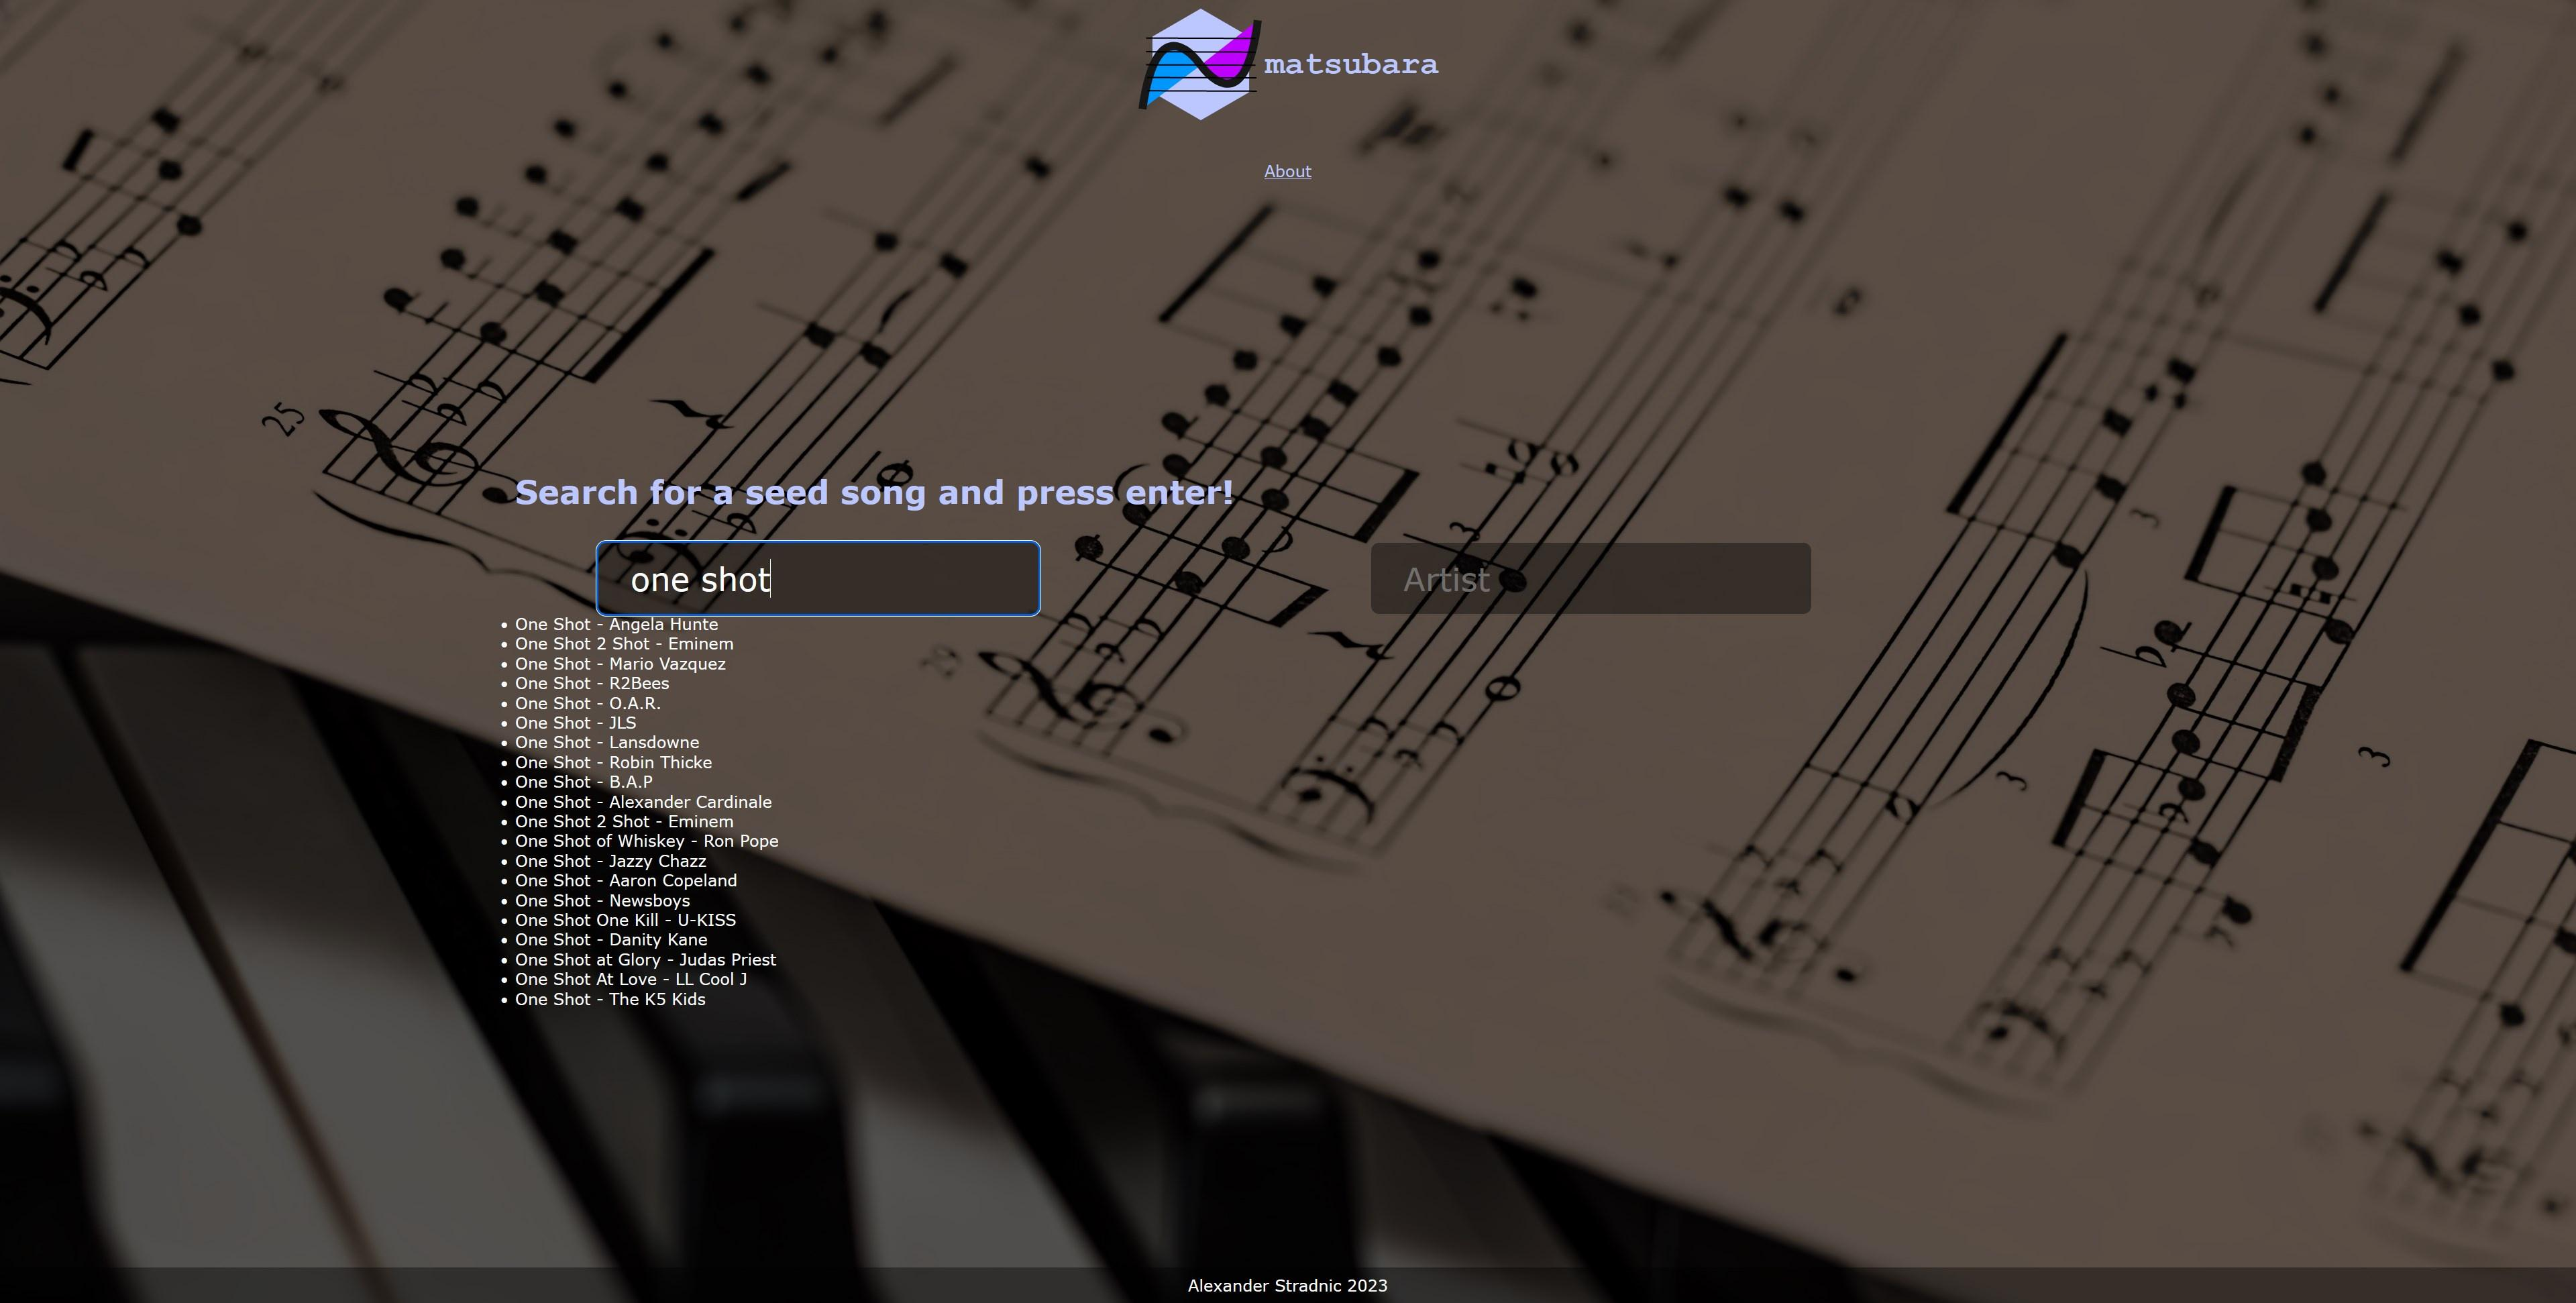
\includegraphics[width=\textwidth]{webapp.jpeg}
\end{figure}

A webapp was developed for the open day and showcases a potential application of the project.
A user chooses their desired song from the list returned after querying a title and/or artist name and is then taken to a screen where they can configure
different settings and options, such as the length of the desired playlist and K amount of input playlists to be factored in. More settings could also be added here.
Multiple algorithms could be configured with different settings.

\begin{figure}[H]
    \centering
    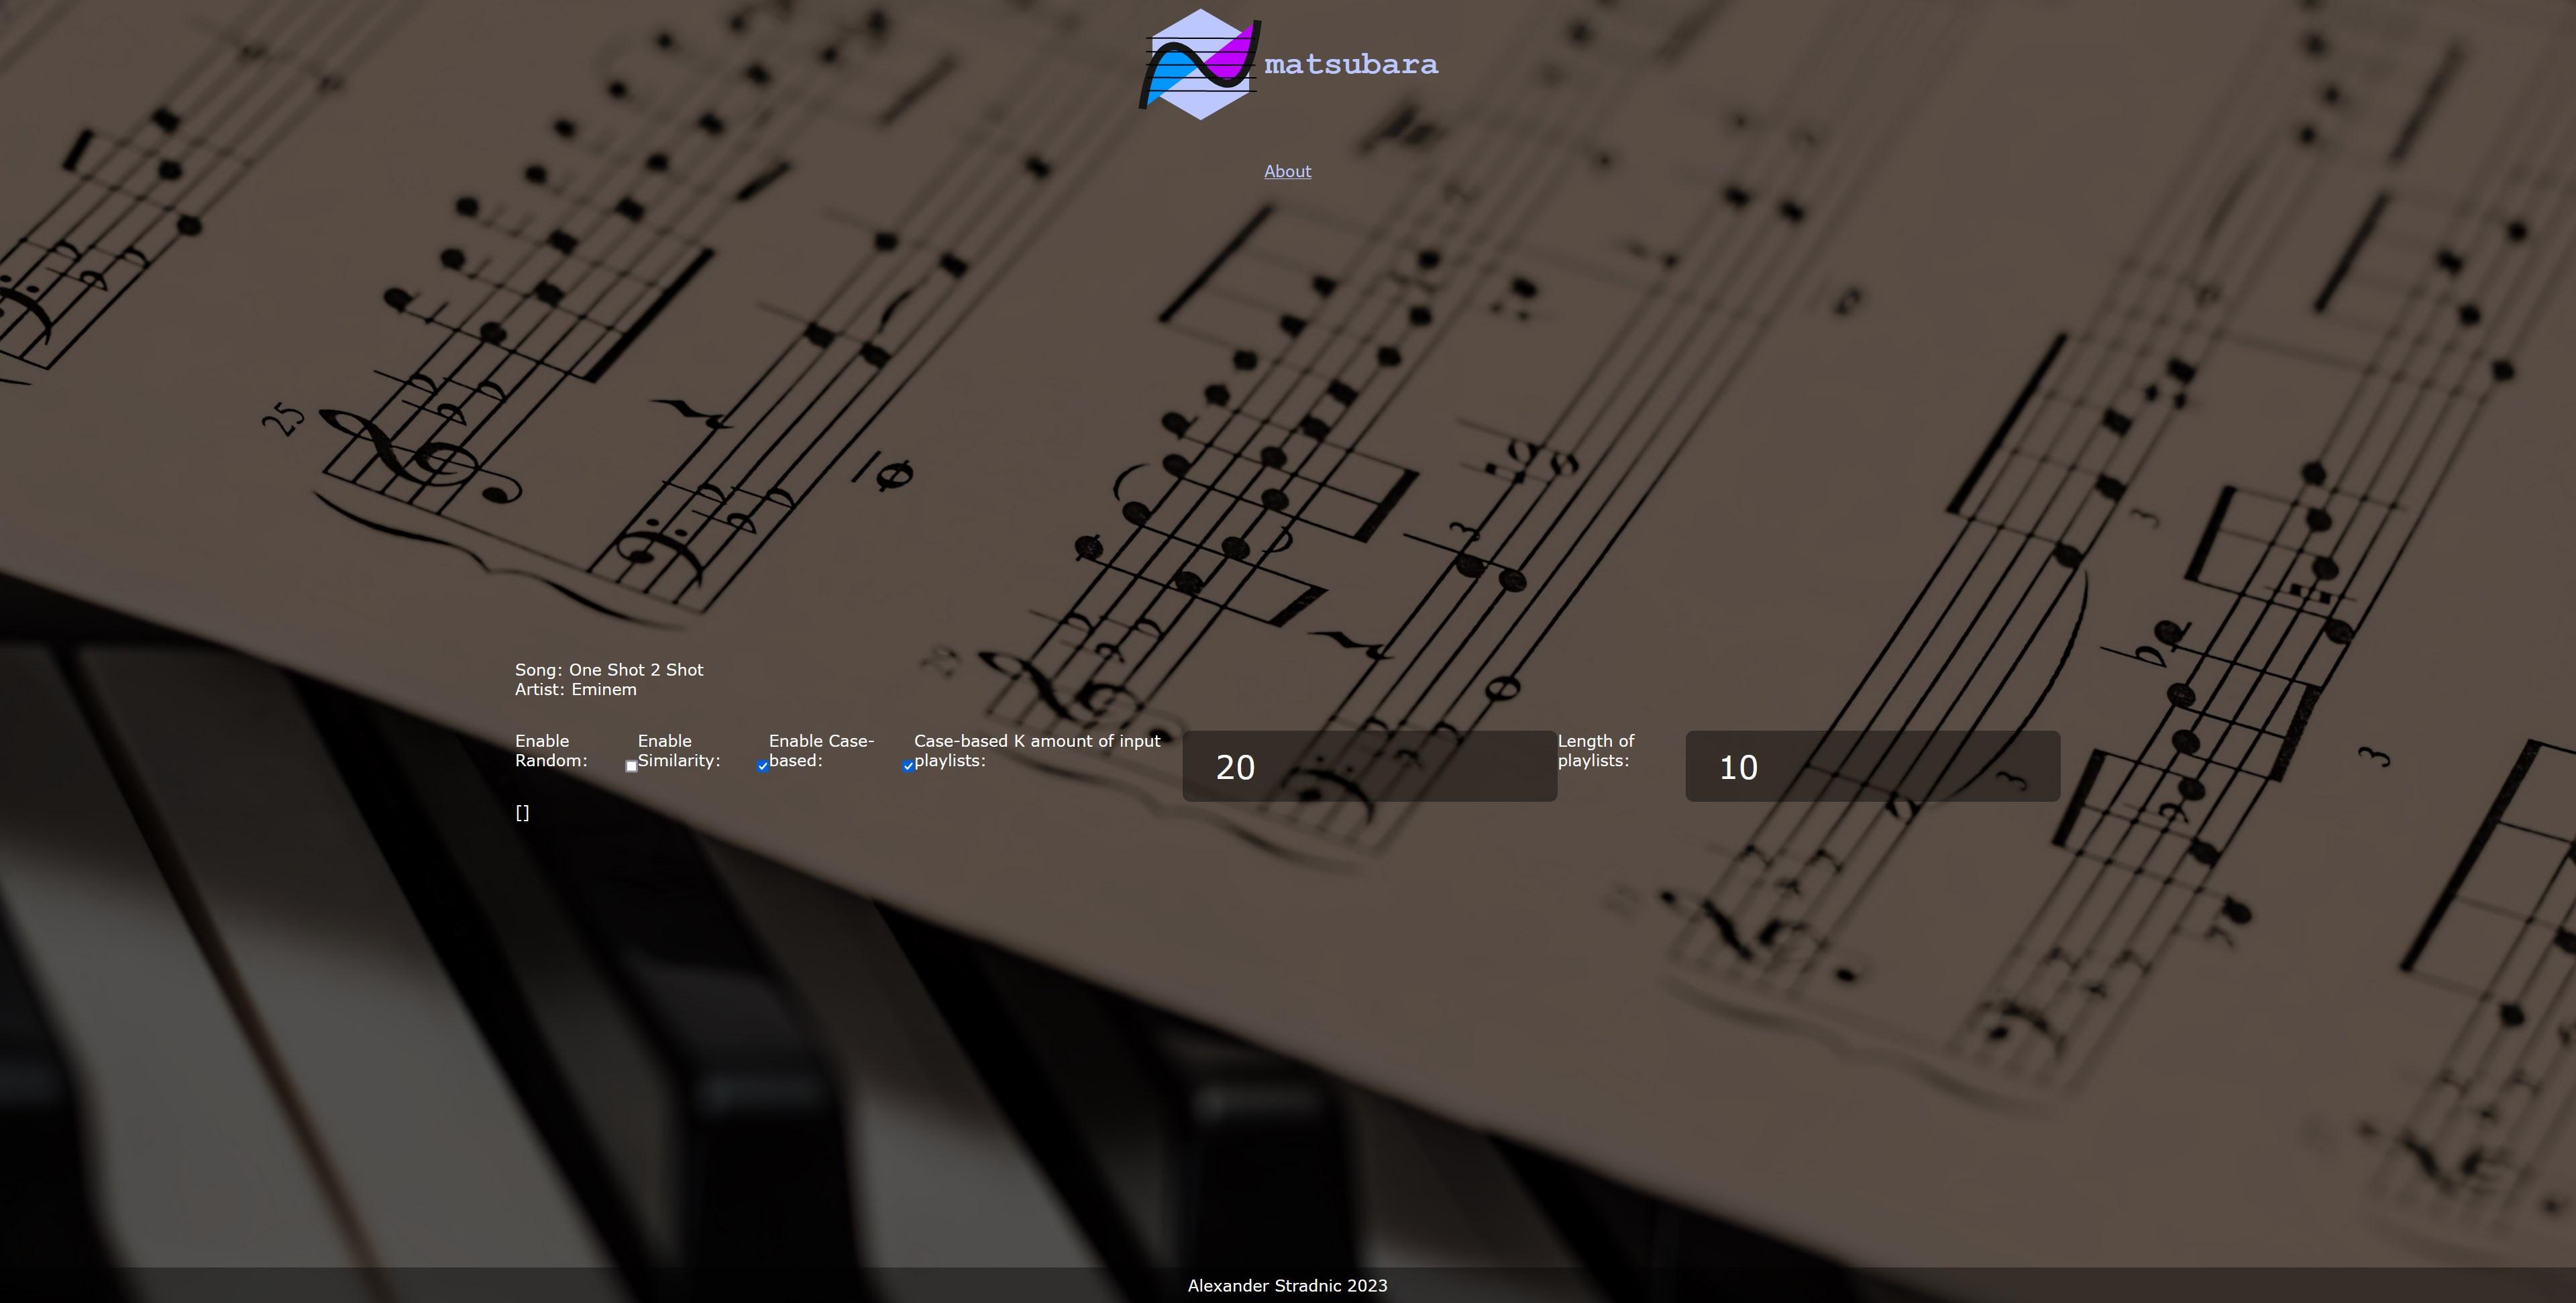
\includegraphics[width=\textwidth]{webapp2.jpeg}
\end{figure}

\subsection*{Further Development}
Unfortunately the main case-based algorithm was not able to output an answer in time due to connection timeout which I did not have the time to solve,
but the premise still works and similarity-based playlists are able to be generated and returned to the client in the form of a list of playlists, each consisting of song URIs.

Song previews could be queried from Spotify on the website, and if a user likes any of the playlists, they could log into their Spotify account
and add them to their profile.

\section{Browser Extension}
Instead of developing a separate website that users have to travel to separately from Spotify, an extension could be developed which a user would simply install,
and would modify the Spotify web client, adding a tab, or simply as a popup like standard browser addons, allowing the user to do the same as above but be
more convenient and even reading context from Spotify. The dataset and program could be downloaded with the addon, allowing local generation instead of pinging a server.

\printbibliography{}

\chapter*{Reference Links}
\normalsize{
\begin{itemize}
    \item Spotify Million Playlist Dataset -- \url{https://engineering.atspotify.com/2018/05/introducing-the-million-playlist-dataset-and-recsys-challenge-2018/}
    \item Spotify Web API Docs -- \url{https://developer.spotify.com/documentation/web-api}
    \\
    \item MusicBrainz -- \url{https://musicbrainz.org/}
    \item Million Song Dataset -- \url{http://millionsongdataset.com/}
    \\
    \item Python Documentation -- \url{https://docs.python.org/3.11/index.html}
    \item SQLite Documentation -- \url{https://www.sqlite.org/doclist.html}
    \item Numpy Documentation -- \url{https://numpy.org/doc/stable/index.html#numpy-docs-mainpage/}
    \item Vue.js Documentation -- \url{https://vuejs.org/guide/introduction.html}
    \item Golang Documentation -- \url{https://go.dev/doc/}
    \\
    \item Sheet Music on Keys Image -- \url{https://www.pexels.com/photo/chords-sheet-on-piano-tiles-210764/}
\end{itemize}
}
\end{document}
